\documentclass{article}
\usepackage[utf8]{inputenc}
\usepackage{hyperref}
\usepackage{listings}
\usepackage{multimedia} % to embed movies in the PDF file
\usepackage{graphicx}
\usepackage{comment}
\usepackage[english]{babel}
\usepackage{amsmath}
\usepackage{amsfonts}
\usepackage{wrapfig}
\usepackage{multirow}
\usepackage{verbatim}
\usepackage{float}
\usepackage{cancel}
\usepackage{caption}
\usepackage{subcaption}
\usepackage{mathdots}
\usepackage{/home/cade/Homework/latex-defs}


\title{AMATH 574 Homework 3}
\author{Cade Ballew \#2120804}
\date{February 2, 2023}

\begin{document}
	
\maketitle
	
\section{Problem 6.1}
We wish to verify that (6.13) results from integrating the linear piecewise solution $\Tilde q^n(x,t_{n+1})=\Tilde q^n(x-\bar u\Delta t,t_n)$. We compute
\begin{align*}
Q^{n+1}_i&=\frac{1}{\Delta x}\int_{\mathcal C_i}\Tilde q^n(x,t_{n+1})dx=\int_{x_{i-1/2}}^{x_{i+1/2}}\Tilde q^n(x-\bar u\Delta t,t_n)dx=\int_{x_{i-1/2}-\bar u\Delta t}^{x_{i+1/2}-\bar u\Delta t}\Tilde q^n(x,t_n)dx\\&=
\frac{1}{\Delta x}\int_{x_{i-1/2}-\bar u\Delta t}^{x_{i-1/2}} \left(Q_{i-1}^n+\sigma_{i-1}^n(x-x_{i-1})\right)dx+\frac{1}{\Delta x}\int_{x_{i-1/2}}^{x_{i+1/2}-\bar u\Delta t} \left(Q_{i}^n+\sigma_{i}^n(x-x_{i})\right)dx\\&=
\frac{\bar u\Delta t}{\Delta x}Q_{i-1}^n+\frac{\sigma_{i-1}^n}{\Delta x}\left[\frac{(x-x_{i-1})^2}{2}\right]_{x_{i-1/2}-\bar u\Delta t}^{x_{i-1/2}}+\frac{\Delta x-\bar u\Delta t}{\Delta x}Q^n_i+\frac{\sigma_{i}^n}{\Delta x}\left[\frac{(x-x_{i})^2}{2}\right]_{x_{i-1/2}}^{x_{i+1/2}-\bar u\Delta t}\\&=
\frac{\bar u\Delta t}{\Delta x}Q_{i-1}^n+\frac{\sigma_{i-1}^n}{\Delta x}\frac{1}{2}\left(\bar u\Delta t\Delta x-(\bar u\Delta t)^2\right)+\left(1-\frac{\bar u\Delta t}{\Delta x}\right)Q^n_i+\frac{\sigma_{i}^n}{\Delta x}\frac{1}{2}\left(-\bar u\Delta t\Delta x+(\bar u\Delta t)^2\right)\\&=
\frac{\bar u\Delta t}{\Delta x}\left(Q_{i-1}^n+\frac{\sigma_{i-1}^n}{2}(\Delta x-\bar u\Delta t)\right)+\frac{\Delta x-\bar u\Delta t}{\Delta x}\left(Q^n_i-\frac{\sigma_{i}^n}{2}\bar u\Delta t\right)
\end{align*}
which of course assumes that $\bar u>0$ a Courant number of no more than one so that the transformed integral only covers two cells. Note that the penultimate line follows from expanding the squares.

\section{Problem 6.4}
Given a function $q$, we define
\[
Q_j=\frac{1}{\Delta x}\int_{\mathcal C_j}q(x)dx
\]
for $j=1,\ldots,N$ which we note is the average  of $q$ over the cell. To show that $\text{TV}(Q)\leq\text{TV}(q)$ we notice that
%\begin{align*}
%|Q_j-Q_{j-1}|=\left|\frac{1}{\Delta x}\int_{\mathcal C_j}q(x)dx-\frac{1}{\Delta x}\int_{\mathcal C_{j-1}}q(x)dx\right|\leq\frac{1}{\Delta x}\int_{\mathcal C_j}\left|q(x)-q(x-\Delta x)\right|dx.
%\end{align*}
%Assuming that the function $|q(x)-q(x-\Delta x)|$ achieves a maximum in the cell $\mathcal C_j$ at some point $y_j$, then,
%\begin{align*}
%\sum_{j=1}^{N}|Q_j-Q_{j-1}|\leq\sum_{j=1}^{N}\frac{1}{\Delta x}\int_{\mathcal C_j}\left|q(y_j)-q(y_j-\Delta x)\right|dx=\sum_{j=1}^N\left|q(y_j)-q(y_j-\Delta x)\right|.
%\end{align*}
$\text{TV}(Q)$ can be computed using the values from the cells where the cell average $Q_j$ has a local maximum or minimum relative to other cell averages. This is because if the averages behave monotonically in a sequence, then the sum of the absolute value of their differences is just the difference of the first and last terms of this sequence. Now, define the sets
\[
m_j=\left\{x\in\mathcal C_j:q(x)\leq Q_j\right\}\quad M_j=\left\{x\in\mathcal C_j:q(x)\geq Q_j\right\}
\]
which are clearly nonempty for any $j$. Now, let $J$ be the set of indices for which $Q_j$ is a local maximum or minimum relative to the other cell averages and denote its elements by $J(1)\leq J(2)\leq\ldots\leq J(M)$. We also let $p_{J(j)}$ be an element from $m_{J(j)}$ if $Q_{J(j)}$ is a local minimum relative to the other cell averages and an element from $M_{J(j)}$ if $Q_{J(j)}$ is a local maximum relative to the other cell averages. Then, we note that $p_{J(1)}\leq p_{J(2)}\leq\ldots\leq p_{J(M)}$ forms a partition of our region, so we have that 
\begin{align*}
\text{TV}(Q)&=\sum_{j=1}^{N}|Q_j-Q_{j-1}|=\sum_{j=1}^{M}\left|Q_{J(j)}-Q_{J(j-1)}\right|\\&
\leq\sum_{j=1}^{M}\left|q(p_{J(j)})-q(p_{J(j-1)})\right|\leq\text{TV}(q)
\end{align*}
since increasing at local maxima and decreasing at local minima can only increase distance between the two, and the total variation of a function is the supremum over all partitions while we have just chosen one.

\section{Problem 6.7}
Consider the case $\bar u<0$ with 
\begin{align*}
&C^n_{i-1}=0,\\
&D^n_i=-\nu+\frac{1}{2}\nu(1+\nu)\left(\phi(\theta_{i+1/2}^n)-\frac{\phi(\theta_{i-1/2}^n)}{\theta_{i-1/2}^n}\right)
\end{align*}
in the context of Theorem 6.1. Plugging this into (6.42), we see that 
\begin{align*}
Q^{n+1}_i&=Q^n_i+\left(-\nu+\frac{1}{2}\nu(1+\nu)\left(\phi(\theta_{i+1/2}^n)-\frac{\phi(\theta_{i-1/2}^n)}{\theta_{i-1/2}^n}\right)\right)(Q^n_{i+1}-Q^n_i)\\&=
Q^n_i-\nu(Q^n_{i+1}-Q^n_i)+\frac{1}{2}\nu(1+\nu)\left(\phi(\theta_{i+1/2}^n)-\phi(\theta_{i-1/2}^n)\frac{Q^n_{i}-Q^n_{i-1}}{Q^n_{i+1}-Q^n_i}\right)(Q^n_{i+1}-Q^n_i)\\&=
Q^n_i-\nu(Q^n_{i+1}-Q^n_i)+\frac{1}{2}\nu(1+\nu)\left(\phi(\theta_{i+1/2}^n)(Q^n_{i+1}-Q^n_i)-\phi(\theta_{i-1/2}^n)(Q^n_{i}-Q^n_{i-1})\right)
\end{align*}
which matches (6.41). Now, we wish to prove that condition (6.43) holds for $\nu\in[-1,0]$. Clearly, the condition that $C^n_{i-1}\geq0$ for all $i$ holds. Note that this choice of $\nu$ implies that $\nu(1+\nu)\leq0$, so assuming the bound (6.44), we have that
\begin{align*}
D^n_i\geq-\nu+\frac{1}{2}\nu(1+\nu)(2)=\nu^2\geq0.
\end{align*}
We also have that 
\begin{align*}
C^n_i+D^n_i\leq-\nu+\frac{1}{2}\nu(1+\nu)(-2)=-\nu^2-2\nu\leq1
\end{align*}
which follows from simple optimization. Thus, this method is in fact TVD.

\section{Problem 8.1}
We wish to perform von Neumann analysis on the method (4.19) for the scalar advection equation $q_t+\bar uq_x=0$. Plugging in the PDE, we have the method
\[
Q^{n+1}_j=Q^n_j-\frac{\bar u\Delta t}{2\Delta x}(Q^n_{j+1}-Q^n_{j-1}).
\]
Let $\Delta t/\Delta x=\mu$ and apply our ansatz $Q^n_j=e^{i\xi j\Delta x}$. Then, we can write
\[
Q^{n+1}_j=\left(1-\frac{\bar u\mu}{2}\left(e^{i\xi\Delta x}-e^{-i\xi\Delta x}\right)\right)Q^n_j=\left(1-i\bar u\mu\sin(\xi\Delta x)\right)Q^n_j.
\]
No matter what choice of $\mu$ we make, $|g|=|1-i\bar u\mu\sin(\xi\Delta x)|\geq1$, and it is always strictly greater than 1 for some $\xi\Delta x$ since $\xi$ is a continuous variable, and sine has isolated zeros. Thus, this method is unstable in the 2-norm for any fixed $\mu=\Delta t/\Delta x$.

\section{Problem 8.9}
We wish to derive the modified equation for the method (4.19) for the scalar advection equation $q_t+\bar uq_x=0$. Letting $v(x,t)=Q^n_i$, we have 
\[
v(x,t+\Delta t)=v(x,t)-\frac{\bar u\Delta t}{2\Delta x}(v(x+\Delta x,t)-v(x-\Delta x,t)).
\]
Taylor expanding,
\begin{align*}
&\text{LHS}=v+\Delta tv_t+\frac{1}{2}(\Delta t)^2v_{tt}+\OO((\Delta t)^3),\\
&\text{RHS}=v-\frac{\bar u\Delta t}{2\Delta x}(2\Delta xv_x+\OO((\Delta x)^3))
\end{align*}
which gives
\[
v_t+\bar uv_x=-\frac{1}{2}\Delta tv_{tt}+\ldots.
\]
Applying the differential equation, we have that 
\[
v_t+\bar uv_x=-\frac{1}{2}\bar{u}^2\Delta tv_{xx}.
\]
Note that this diffision coefficient is always negative no matter if $\bar u>0$ or $\bar u<0$, so the modified equation is ill-posed.

\section{Problem 7.2}
\subsection{Part a}
We wish to solve a Riemann problem at $x_{1/2}=a$ with data 
\[
Q_0=\begin{pmatrix}
	p_1\\-u_1
\end{pmatrix},\quad Q_1=\begin{pmatrix}
p_1\\u_1
\end{pmatrix}
\]
for the acoustics equation which corresponds to the ghost-cell values (7.17). Recall from (2.66) that this equation has inverse eigenvector matrix 
\[
R^{-1}=\frac{1}{2Z_0}\begin{pmatrix}
	-1 &Z_0\\
	1&Z_0
\end{pmatrix},
\]
so we can compute
\[
\alpha=R^{-1}(Q_1-Q_0)=\frac{1}{2Z_0}\begin{pmatrix}
	-1 &Z_0\\
	1&Z_0
\end{pmatrix}\begin{pmatrix}
0\\2u_1
\end{pmatrix}=\begin{pmatrix}
u_1\\u_1
\end{pmatrix}.
\]
Then, the intermediate state is given by
\[
q^*=Q_0+\alpha^1r^1=\begin{pmatrix}
	p_1\\-u_1
\end{pmatrix}+u_1\begin{pmatrix}
-Z_0\\1
\end{pmatrix}=\begin{pmatrix}
p_1-u_1Z_0\\0
\end{pmatrix},
\]
so $u^*=0$ along the wall as expected.
\subsection{Part b}
If we instead wish to the same Riemann problem but with data  
\[
Q_0=\begin{pmatrix}
	p_1\\2U(t_n)-u_1
\end{pmatrix},\quad Q_1=\begin{pmatrix}
	p_1\\u_1
\end{pmatrix}
\]
corresponding to oscillating-wall boundary conditions (7.20), we instead get that 
\[
\alpha=\frac{1}{2Z_0}\begin{pmatrix}
	-1 &Z_0\\
	1&Z_0
\end{pmatrix}\begin{pmatrix}
	0\\2U(t_n)+2u_1
\end{pmatrix}=\begin{pmatrix}
	u_1\\U(t_n)+u_1
\end{pmatrix},
\]
so the intermediate state is given by
\[
q^*=Q_0+\alpha^1r^1=\begin{pmatrix}
	p_1\\U(t_n)-u_1
\end{pmatrix}+u_1\begin{pmatrix}
	-Z_0\\1
\end{pmatrix}=\begin{pmatrix}
	p_1-u_1Z_0\\U(t_n)
\end{pmatrix}
\]
which again matches our boundary condition as expected.

\section{Problem 7.3}
In the default settings for a standing wave in Clawpack, the acoustics equations are solved for solid wall boundary conditions, meaning that the behavior should be as described in example 3.2 in which this is discussed. At both boundaries, we expect outgoing waves to be completely reflected and to feed back into the incoming waves. This is precisely what we observe in the figures for both pressure and velocity. \\
We modify this by instead considering zero-order extrapolation at the right boundary which corresponds to outflow. We expect the behavior to be as in Figure 3.8 where waves are completely reflected and to feed back into the incoming waves on the left boundary as before, but right-going waves leave the domain with no reflection. This behavior is particularly apparent when the simulation is run backwards in time. We now include some of the outputted plots which exhibit this.\\
\begin{figure}[H]
	\centering
	\begin{subfigure}{0.495\linewidth}
		\centering
		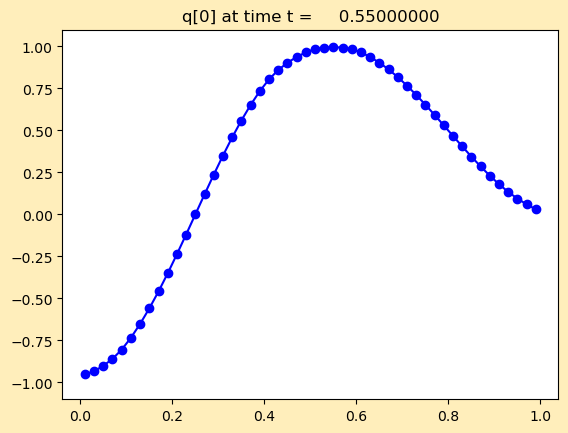
\includegraphics[width=\linewidth]{standing/_plots/frame0011fig0.png}
	\end{subfigure}
	\begin{subfigure}{0.495\linewidth}
		\centering
		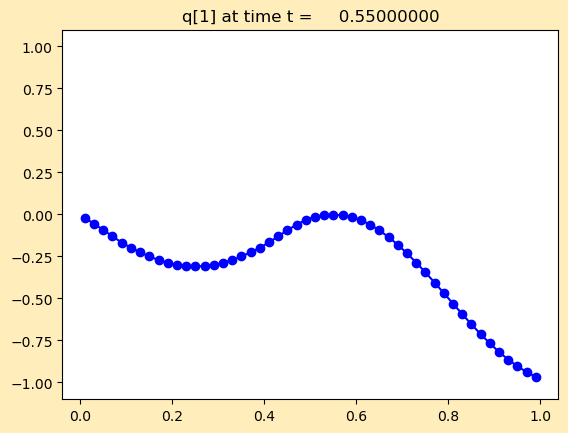
\includegraphics[width=\linewidth]{standing/_plots/frame0011fig1.png}
	\end{subfigure}
	\centering
	\begin{subfigure}{0.495\linewidth}
		\centering
		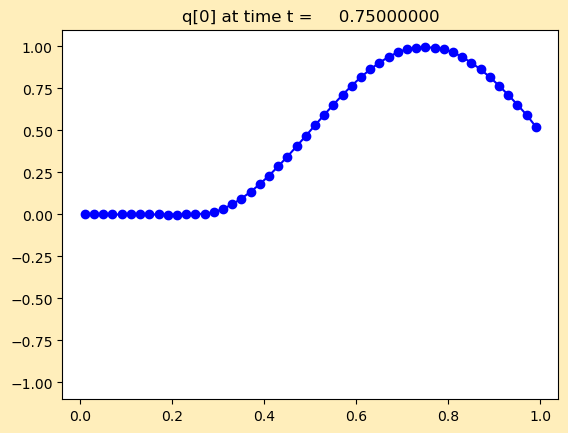
\includegraphics[width=\linewidth]{standing/_plots/frame0015fig0.png}
	\end{subfigure}
	\begin{subfigure}{0.495\linewidth}
		\centering
		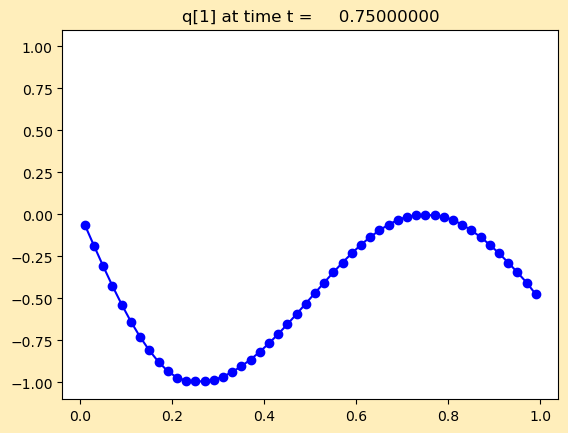
\includegraphics[width=\linewidth]{standing/_plots/frame0015fig1.png}
	\end{subfigure}
\end{figure}
\begin{figure}[H]
	\centering
	\begin{subfigure}{0.495\linewidth}
		\centering
		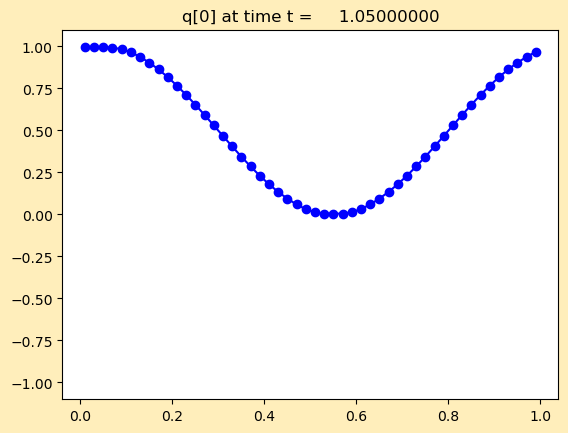
\includegraphics[width=\linewidth]{standing/_plots/frame0021fig0.png}
	\end{subfigure}
	\begin{subfigure}{0.495\linewidth}
		\centering
		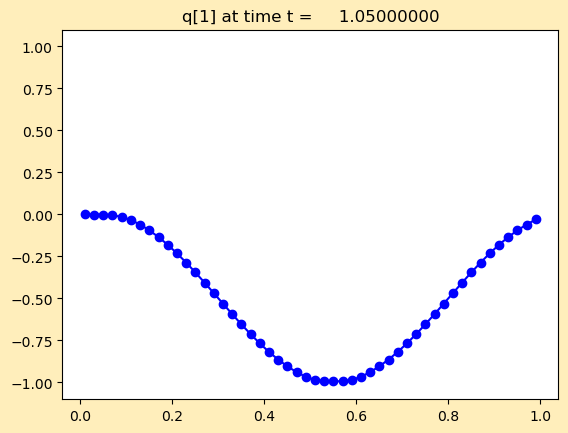
\includegraphics[width=\linewidth]{standing/_plots/frame0021fig1.png}
	\end{subfigure}
	\centering
	\begin{subfigure}{0.495\linewidth}
		\centering
		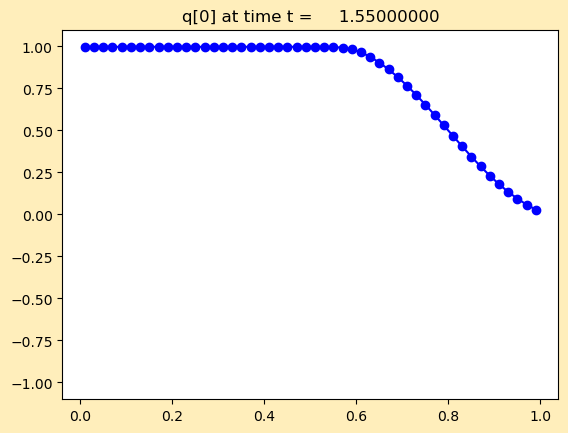
\includegraphics[width=\linewidth]{standing/_plots/frame0031fig0.png}
	\end{subfigure}
	\begin{subfigure}{0.495\linewidth}
		\centering
		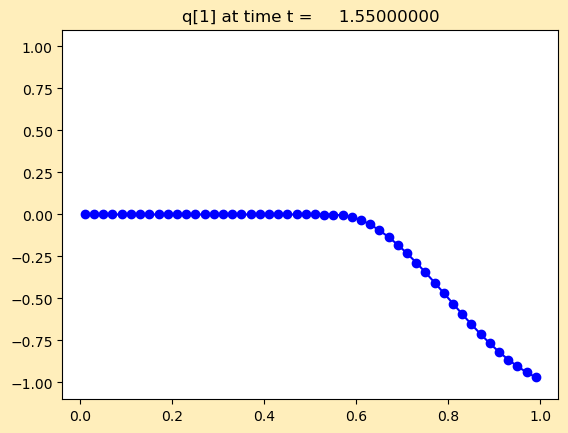
\includegraphics[width=\linewidth]{standing/_plots/frame0031fig1.png}
	\end{subfigure}
\end{figure}

\end{document}
